% Options for packages loaded elsewhere
\PassOptionsToPackage{unicode}{hyperref}
\PassOptionsToPackage{hyphens}{url}
%
\documentclass[
]{article}
\title{Homework 2}
\author{Skasko\_Stephen}
\date{2023-02-03}

\usepackage{amsmath,amssymb}
\usepackage{lmodern}
\usepackage{iftex}
\ifPDFTeX
  \usepackage[T1]{fontenc}
  \usepackage[utf8]{inputenc}
  \usepackage{textcomp} % provide euro and other symbols
\else % if luatex or xetex
  \usepackage{unicode-math}
  \defaultfontfeatures{Scale=MatchLowercase}
  \defaultfontfeatures[\rmfamily]{Ligatures=TeX,Scale=1}
\fi
% Use upquote if available, for straight quotes in verbatim environments
\IfFileExists{upquote.sty}{\usepackage{upquote}}{}
\IfFileExists{microtype.sty}{% use microtype if available
  \usepackage[]{microtype}
  \UseMicrotypeSet[protrusion]{basicmath} % disable protrusion for tt fonts
}{}
\makeatletter
\@ifundefined{KOMAClassName}{% if non-KOMA class
  \IfFileExists{parskip.sty}{%
    \usepackage{parskip}
  }{% else
    \setlength{\parindent}{0pt}
    \setlength{\parskip}{6pt plus 2pt minus 1pt}}
}{% if KOMA class
  \KOMAoptions{parskip=half}}
\makeatother
\usepackage{xcolor}
\IfFileExists{xurl.sty}{\usepackage{xurl}}{} % add URL line breaks if available
\IfFileExists{bookmark.sty}{\usepackage{bookmark}}{\usepackage{hyperref}}
\hypersetup{
  pdftitle={Homework 2},
  pdfauthor={Skasko\_Stephen},
  hidelinks,
  pdfcreator={LaTeX via pandoc}}
\urlstyle{same} % disable monospaced font for URLs
\usepackage[margin=1in]{geometry}
\usepackage{color}
\usepackage{fancyvrb}
\newcommand{\VerbBar}{|}
\newcommand{\VERB}{\Verb[commandchars=\\\{\}]}
\DefineVerbatimEnvironment{Highlighting}{Verbatim}{commandchars=\\\{\}}
% Add ',fontsize=\small' for more characters per line
\usepackage{framed}
\definecolor{shadecolor}{RGB}{248,248,248}
\newenvironment{Shaded}{\begin{snugshade}}{\end{snugshade}}
\newcommand{\AlertTok}[1]{\textcolor[rgb]{0.94,0.16,0.16}{#1}}
\newcommand{\AnnotationTok}[1]{\textcolor[rgb]{0.56,0.35,0.01}{\textbf{\textit{#1}}}}
\newcommand{\AttributeTok}[1]{\textcolor[rgb]{0.77,0.63,0.00}{#1}}
\newcommand{\BaseNTok}[1]{\textcolor[rgb]{0.00,0.00,0.81}{#1}}
\newcommand{\BuiltInTok}[1]{#1}
\newcommand{\CharTok}[1]{\textcolor[rgb]{0.31,0.60,0.02}{#1}}
\newcommand{\CommentTok}[1]{\textcolor[rgb]{0.56,0.35,0.01}{\textit{#1}}}
\newcommand{\CommentVarTok}[1]{\textcolor[rgb]{0.56,0.35,0.01}{\textbf{\textit{#1}}}}
\newcommand{\ConstantTok}[1]{\textcolor[rgb]{0.00,0.00,0.00}{#1}}
\newcommand{\ControlFlowTok}[1]{\textcolor[rgb]{0.13,0.29,0.53}{\textbf{#1}}}
\newcommand{\DataTypeTok}[1]{\textcolor[rgb]{0.13,0.29,0.53}{#1}}
\newcommand{\DecValTok}[1]{\textcolor[rgb]{0.00,0.00,0.81}{#1}}
\newcommand{\DocumentationTok}[1]{\textcolor[rgb]{0.56,0.35,0.01}{\textbf{\textit{#1}}}}
\newcommand{\ErrorTok}[1]{\textcolor[rgb]{0.64,0.00,0.00}{\textbf{#1}}}
\newcommand{\ExtensionTok}[1]{#1}
\newcommand{\FloatTok}[1]{\textcolor[rgb]{0.00,0.00,0.81}{#1}}
\newcommand{\FunctionTok}[1]{\textcolor[rgb]{0.00,0.00,0.00}{#1}}
\newcommand{\ImportTok}[1]{#1}
\newcommand{\InformationTok}[1]{\textcolor[rgb]{0.56,0.35,0.01}{\textbf{\textit{#1}}}}
\newcommand{\KeywordTok}[1]{\textcolor[rgb]{0.13,0.29,0.53}{\textbf{#1}}}
\newcommand{\NormalTok}[1]{#1}
\newcommand{\OperatorTok}[1]{\textcolor[rgb]{0.81,0.36,0.00}{\textbf{#1}}}
\newcommand{\OtherTok}[1]{\textcolor[rgb]{0.56,0.35,0.01}{#1}}
\newcommand{\PreprocessorTok}[1]{\textcolor[rgb]{0.56,0.35,0.01}{\textit{#1}}}
\newcommand{\RegionMarkerTok}[1]{#1}
\newcommand{\SpecialCharTok}[1]{\textcolor[rgb]{0.00,0.00,0.00}{#1}}
\newcommand{\SpecialStringTok}[1]{\textcolor[rgb]{0.31,0.60,0.02}{#1}}
\newcommand{\StringTok}[1]{\textcolor[rgb]{0.31,0.60,0.02}{#1}}
\newcommand{\VariableTok}[1]{\textcolor[rgb]{0.00,0.00,0.00}{#1}}
\newcommand{\VerbatimStringTok}[1]{\textcolor[rgb]{0.31,0.60,0.02}{#1}}
\newcommand{\WarningTok}[1]{\textcolor[rgb]{0.56,0.35,0.01}{\textbf{\textit{#1}}}}
\usepackage{graphicx}
\makeatletter
\def\maxwidth{\ifdim\Gin@nat@width>\linewidth\linewidth\else\Gin@nat@width\fi}
\def\maxheight{\ifdim\Gin@nat@height>\textheight\textheight\else\Gin@nat@height\fi}
\makeatother
% Scale images if necessary, so that they will not overflow the page
% margins by default, and it is still possible to overwrite the defaults
% using explicit options in \includegraphics[width, height, ...]{}
\setkeys{Gin}{width=\maxwidth,height=\maxheight,keepaspectratio}
% Set default figure placement to htbp
\makeatletter
\def\fps@figure{htbp}
\makeatother
\setlength{\emergencystretch}{3em} % prevent overfull lines
\providecommand{\tightlist}{%
  \setlength{\itemsep}{0pt}\setlength{\parskip}{0pt}}
\setcounter{secnumdepth}{-\maxdimen} % remove section numbering
\ifLuaTeX
  \usepackage{selnolig}  % disable illegal ligatures
\fi

\begin{document}
\maketitle

\hypertarget{section}{%
\subsection{1.}\label{section}}

Work through all of the labs given in Section 3.6 of the ISLR textbook.
Make sure that you are extremely comfortable with the lm function and
how to obtain each type of output discussed. Pay particular attention to
the final two Sections (3.6.6 - 3.6.7) as many of your projects will
involve understanding how categorical predictors are treated (3.6.6) and
writing your own functions in R (3.6.7) is something that nearly always
needs done when writing larger programs. You do not need to turn
anything in for this.

\hypertarget{section-1}{%
\subsection{2.}\label{section-1}}

\hypertarget{chapter-3-conceptual-exercise-3}{%
\subsection{Chapter 3 Conceptual Exercise
3}\label{chapter-3-conceptual-exercise-3}}

\hypertarget{a}{%
\subsubsection{(a)}\label{a}}

\hypertarget{i.}{%
\subsubsection{i.}\label{i.}}

\hypertarget{ii.}{%
\subsubsection{ii.}\label{ii.}}

\hypertarget{iii.}{%
\subsubsection{iii.}\label{iii.}}

35-10x1\textgreater= 0 --\textgreater{} x1 \textgreater= 3.5

High school graduates on average make more when their GPA is higher or
equal to 3.5

\hypertarget{iv.}{%
\subsubsection{iv.}\label{iv.}}

\hypertarget{b}{%
\subsubsection{(b)}\label{b}}

S = 50 + 20(4) + 0.07(110) + 35 + 0.01(110*4) - 10(4) = 137.1

\hypertarget{c}{%
\subsubsection{(c)}\label{c}}

False, based on the coefficient size does not indicate a significance of
data.

\hypertarget{chapter-3-conceptual-exercise-4}{%
\subsection{Chapter 3 Conceptual Exercise
4}\label{chapter-3-conceptual-exercise-4}}

\hypertarget{a-1}{%
\subsubsection{(a)}\label{a-1}}

Expected to be lower since it would better fit the data with a bigger
irreducible error \#\#\# (b) Expect to be higher as the overfitting from
training of the model would have more error \#\#\# (c) Expect to be
lower because of high flexibility \#\#\# (d) I don't believe we have
enough information for this because we are unsure about the true
relationship or linearity \#\# 3. \#\# Chapter 3 Applied Exercise 9

\hypertarget{a-2}{%
\subsubsection{(a)}\label{a-2}}

\begin{Shaded}
\begin{Highlighting}[]
\FunctionTok{library}\NormalTok{(ISLR2)}
\FunctionTok{pairs}\NormalTok{(Auto)}
\end{Highlighting}
\end{Shaded}

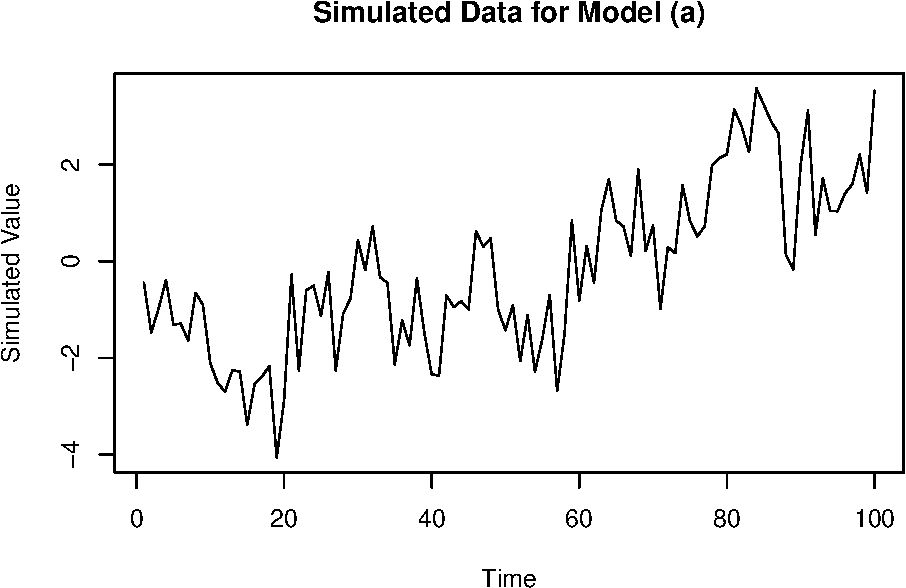
\includegraphics{Homework_2_Template_files/figure-latex/unnamed-chunk-1-1.pdf}

\hypertarget{b-1}{%
\subsubsection{(b)}\label{b-1}}

\begin{Shaded}
\begin{Highlighting}[]
\CommentTok{\#names(Auto)}
\FunctionTok{cor}\NormalTok{(Auto[,}\SpecialCharTok{{-}}\DecValTok{9}\NormalTok{])}
\end{Highlighting}
\end{Shaded}

\begin{verbatim}
##                     mpg  cylinders displacement horsepower     weight
## mpg           1.0000000 -0.7776175   -0.8051269 -0.7784268 -0.8322442
## cylinders    -0.7776175  1.0000000    0.9508233  0.8429834  0.8975273
## displacement -0.8051269  0.9508233    1.0000000  0.8972570  0.9329944
## horsepower   -0.7784268  0.8429834    0.8972570  1.0000000  0.8645377
## weight       -0.8322442  0.8975273    0.9329944  0.8645377  1.0000000
## acceleration  0.4233285 -0.5046834   -0.5438005 -0.6891955 -0.4168392
## year          0.5805410 -0.3456474   -0.3698552 -0.4163615 -0.3091199
## origin        0.5652088 -0.5689316   -0.6145351 -0.4551715 -0.5850054
##              acceleration       year     origin
## mpg             0.4233285  0.5805410  0.5652088
## cylinders      -0.5046834 -0.3456474 -0.5689316
## displacement   -0.5438005 -0.3698552 -0.6145351
## horsepower     -0.6891955 -0.4163615 -0.4551715
## weight         -0.4168392 -0.3091199 -0.5850054
## acceleration    1.0000000  0.2903161  0.2127458
## year            0.2903161  1.0000000  0.1815277
## origin          0.2127458  0.1815277  1.0000000
\end{verbatim}

\hypertarget{c-1}{%
\subsubsection{(c)}\label{c-1}}

i: Yes because since predictors have a relationship with the response
based on the p-values. ii: Predictors: Displacement, weight, year, and
origin who do have a statistically significant relationship to the
response iii: Shows that the coefficient of every 3-4 years goes up by 3
mpg

\begin{Shaded}
\begin{Highlighting}[]
\NormalTok{rid }\OtherTok{\textless{}{-}}\NormalTok{ Auto[, }\SpecialCharTok{{-}}\DecValTok{9}\NormalTok{]}


\NormalTok{model }\OtherTok{\textless{}{-}} \FunctionTok{lm}\NormalTok{(mpg }\SpecialCharTok{\textasciitilde{}}\NormalTok{ .,  }\AttributeTok{data =}\NormalTok{ rid)}
\FunctionTok{summary}\NormalTok{(model)}
\end{Highlighting}
\end{Shaded}

\begin{verbatim}
## 
## Call:
## lm(formula = mpg ~ ., data = rid)
## 
## Residuals:
##     Min      1Q  Median      3Q     Max 
## -9.5903 -2.1565 -0.1169  1.8690 13.0604 
## 
## Coefficients:
##                Estimate Std. Error t value Pr(>|t|)    
## (Intercept)  -17.218435   4.644294  -3.707  0.00024 ***
## cylinders     -0.493376   0.323282  -1.526  0.12780    
## displacement   0.019896   0.007515   2.647  0.00844 ** 
## horsepower    -0.016951   0.013787  -1.230  0.21963    
## weight        -0.006474   0.000652  -9.929  < 2e-16 ***
## acceleration   0.080576   0.098845   0.815  0.41548    
## year           0.750773   0.050973  14.729  < 2e-16 ***
## origin         1.426141   0.278136   5.127 4.67e-07 ***
## ---
## Signif. codes:  0 '***' 0.001 '**' 0.01 '*' 0.05 '.' 0.1 ' ' 1
## 
## Residual standard error: 3.328 on 384 degrees of freedom
## Multiple R-squared:  0.8215, Adjusted R-squared:  0.8182 
## F-statistic: 252.4 on 7 and 384 DF,  p-value: < 2.2e-16
\end{verbatim}

\hypertarget{d}{%
\subsubsection{(d)}\label{d}}

Problems: Shows heteroscedasticity in graph, non-linearity, high
leverage points, but most outliers seem contained except for the last
graph at 14.

\begin{Shaded}
\begin{Highlighting}[]
\FunctionTok{plot}\NormalTok{(model)}
\end{Highlighting}
\end{Shaded}

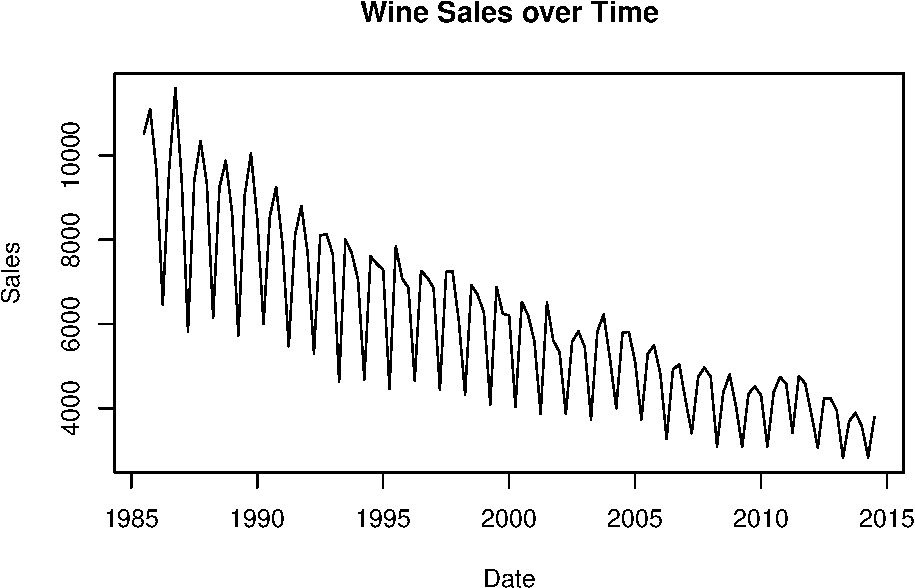
\includegraphics{Homework_2_Template_files/figure-latex/unnamed-chunk-4-1.pdf}
\includegraphics{Homework_2_Template_files/figure-latex/unnamed-chunk-4-2.pdf}
\includegraphics{Homework_2_Template_files/figure-latex/unnamed-chunk-4-3.pdf}
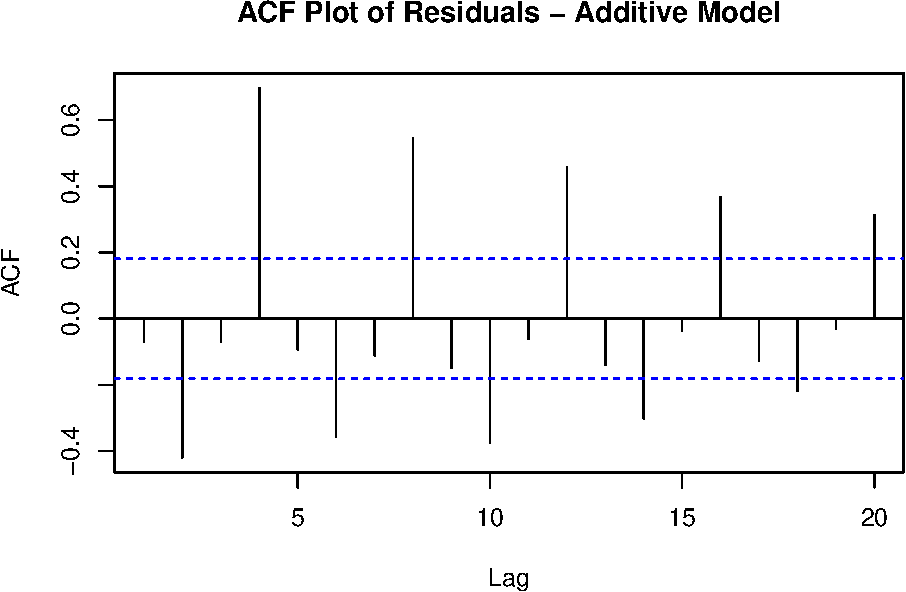
\includegraphics{Homework_2_Template_files/figure-latex/unnamed-chunk-4-4.pdf}

\hypertarget{e}{%
\subsubsection{(e)}\label{e}}

Interaction terms: Displacement * horsepower, horsepower*origin

More interactions means more decrease in the significant values

\begin{Shaded}
\begin{Highlighting}[]
\NormalTok{fit }\OtherTok{\textless{}{-}} \FunctionTok{lm}\NormalTok{(mpg }\SpecialCharTok{\textasciitilde{}}\NormalTok{ . }\SpecialCharTok{+}\NormalTok{ horsepower}\SpecialCharTok{*}\NormalTok{origin }\SpecialCharTok{+}\NormalTok{ horsepower}\SpecialCharTok{*}\NormalTok{displacement }\SpecialCharTok{{-}}\NormalTok{ name, }\AttributeTok{data =}\NormalTok{ Auto)}
\FunctionTok{summary}\NormalTok{(fit)}
\end{Highlighting}
\end{Shaded}

\begin{verbatim}
## 
## Call:
## lm(formula = mpg ~ . + horsepower * origin + horsepower * displacement - 
##     name, data = Auto)
## 
## Residuals:
##     Min      1Q  Median      3Q     Max 
## -8.7222 -1.5251 -0.0968  1.3553 12.8419 
## 
## Coefficients:
##                           Estimate Std. Error t value Pr(>|t|)    
## (Intercept)             -4.706e+00  4.686e+00  -1.004   0.3159    
## cylinders                5.142e-01  3.139e-01   1.638   0.1022    
## displacement            -6.970e-02  1.143e-02  -6.098 2.63e-09 ***
## horsepower              -1.540e-01  3.547e-02  -4.342 1.81e-05 ***
## weight                  -3.084e-03  6.478e-04  -4.761 2.73e-06 ***
## acceleration            -2.276e-01  9.099e-02  -2.501   0.0128 *  
## year                     7.349e-01  4.460e-02  16.478  < 2e-16 ***
## origin                   2.281e+00  1.090e+00   2.092   0.0371 *  
## horsepower:origin       -1.918e-02  1.278e-02  -1.500   0.1343    
## displacement:horsepower  4.665e-04  6.127e-05   7.614 2.10e-13 ***
## ---
## Signif. codes:  0 '***' 0.001 '**' 0.01 '*' 0.05 '.' 0.1 ' ' 1
## 
## Residual standard error: 2.908 on 382 degrees of freedom
## Multiple R-squared:  0.8644, Adjusted R-squared:  0.8612 
## F-statistic: 270.6 on 9 and 382 DF,  p-value: < 2.2e-16
\end{verbatim}

\hypertarget{f}{%
\subsubsection{(f)}\label{f}}

Similarities between p-values and high F-statistics. Another interesting
thing is that origin has a higher value overall and most of the values
are less than or around 1 except origin.

\begin{Shaded}
\begin{Highlighting}[]
\NormalTok{model\_new1 }\OtherTok{\textless{}{-}} \FunctionTok{lm}\NormalTok{(mpg }\SpecialCharTok{\textasciitilde{}}\NormalTok{ . }\SpecialCharTok{+} \FunctionTok{log}\NormalTok{(weight), }\AttributeTok{data =}\NormalTok{ Auto[}\SpecialCharTok{{-}}\DecValTok{9}\NormalTok{])}
\FunctionTok{summary}\NormalTok{(model\_new1)}
\end{Highlighting}
\end{Shaded}

\begin{verbatim}
## 
## Call:
## lm(formula = mpg ~ . + log(weight), data = Auto[-9])
## 
## Residuals:
##     Min      1Q  Median      3Q     Max 
## -9.6516 -1.6398 -0.1671  1.5973 12.7247 
## 
## Coefficients:
##                Estimate Std. Error t value Pr(>|t|)    
## (Intercept)  269.474171  31.136919   8.654  < 2e-16 ***
## cylinders     -0.498204   0.292415  -1.704  0.08924 .  
## displacement   0.013527   0.006832   1.980  0.04843 *  
## horsepower    -0.022137   0.012483  -1.773  0.07696 .  
## weight         0.007657   0.001631   4.694 3.73e-06 ***
## acceleration   0.045763   0.089486   0.511  0.60936    
## year           0.797808   0.046383  17.200  < 2e-16 ***
## origin         0.719552   0.262819   2.738  0.00647 ** 
## log(weight)  -41.320927   4.446725  -9.292  < 2e-16 ***
## ---
## Signif. codes:  0 '***' 0.001 '**' 0.01 '*' 0.05 '.' 0.1 ' ' 1
## 
## Residual standard error: 3.01 on 383 degrees of freedom
## Multiple R-squared:  0.8543, Adjusted R-squared:  0.8513 
## F-statistic: 280.8 on 8 and 383 DF,  p-value: < 2.2e-16
\end{verbatim}

\begin{Shaded}
\begin{Highlighting}[]
\NormalTok{model\_new2 }\OtherTok{\textless{}{-}} \FunctionTok{lm}\NormalTok{(mpg }\SpecialCharTok{\textasciitilde{}}\NormalTok{ . }\SpecialCharTok{+} \FunctionTok{sqrt}\NormalTok{(horsepower}\SpecialCharTok{\^{}}\DecValTok{2}\NormalTok{) }\SpecialCharTok{+}\NormalTok{ mpg, }\AttributeTok{data =}\NormalTok{ Auto[}\SpecialCharTok{{-}}\DecValTok{9}\NormalTok{])}
\end{Highlighting}
\end{Shaded}

\begin{verbatim}
## Warning in model.matrix.default(mt, mf, contrasts): the response appeared on the
## right-hand side and was dropped
\end{verbatim}

\begin{verbatim}
## Warning in model.matrix.default(mt, mf, contrasts): problem with term 9 in
## model.matrix: no columns are assigned
\end{verbatim}

\begin{Shaded}
\begin{Highlighting}[]
\FunctionTok{summary}\NormalTok{(model\_new2)}
\end{Highlighting}
\end{Shaded}

\begin{verbatim}
## 
## Call:
## lm(formula = mpg ~ . + sqrt(horsepower^2) + mpg, data = Auto[-9])
## 
## Residuals:
##     Min      1Q  Median      3Q     Max 
## -9.5903 -2.1565 -0.1169  1.8690 13.0604 
## 
## Coefficients: (1 not defined because of singularities)
##                      Estimate Std. Error t value Pr(>|t|)    
## (Intercept)        -17.218435   4.644294  -3.707  0.00024 ***
## cylinders           -0.493376   0.323282  -1.526  0.12780    
## displacement         0.019896   0.007515   2.647  0.00844 ** 
## horsepower          -0.016951   0.013787  -1.230  0.21963    
## weight              -0.006474   0.000652  -9.929  < 2e-16 ***
## acceleration         0.080576   0.098845   0.815  0.41548    
## year                 0.750773   0.050973  14.729  < 2e-16 ***
## origin               1.426141   0.278136   5.127 4.67e-07 ***
## sqrt(horsepower^2)         NA         NA      NA       NA    
## ---
## Signif. codes:  0 '***' 0.001 '**' 0.01 '*' 0.05 '.' 0.1 ' ' 1
## 
## Residual standard error: 3.328 on 384 degrees of freedom
## Multiple R-squared:  0.8215, Adjusted R-squared:  0.8182 
## F-statistic: 252.4 on 7 and 384 DF,  p-value: < 2.2e-16
\end{verbatim}

\begin{Shaded}
\begin{Highlighting}[]
\NormalTok{model\_new3 }\OtherTok{\textless{}{-}} \FunctionTok{lm}\NormalTok{(mpg }\SpecialCharTok{\textasciitilde{}}\NormalTok{ . }\SpecialCharTok{+} \FunctionTok{I}\NormalTok{(acceleration}\SpecialCharTok{\^{}}\DecValTok{2}\NormalTok{), }\AttributeTok{data =}\NormalTok{ Auto[}\SpecialCharTok{{-}}\DecValTok{9}\NormalTok{])}
\FunctionTok{summary}\NormalTok{(model\_new3)}
\end{Highlighting}
\end{Shaded}

\begin{verbatim}
## 
## Call:
## lm(formula = mpg ~ . + I(acceleration^2), data = Auto[-9])
## 
## Residuals:
##     Min      1Q  Median      3Q     Max 
## -9.9680 -1.9266 -0.0124  1.9153 13.2722 
## 
## Coefficients:
##                     Estimate Std. Error t value Pr(>|t|)    
## (Intercept)        5.1088174  6.4930423   0.787   0.4319    
## cylinders         -0.3181584  0.3165577  -1.005   0.3155    
## displacement       0.0090446  0.0076528   1.182   0.2380    
## horsepower        -0.0346411  0.0139094  -2.490   0.0132 *  
## weight            -0.0054113  0.0006719  -8.053 1.03e-14 ***
## acceleration      -2.6374431  0.5758788  -4.580 6.30e-06 ***
## year               0.7535781  0.0495815  15.199  < 2e-16 ***
## origin             1.3265929  0.2713219   4.889 1.49e-06 ***
## I(acceleration^2)  0.0790472  0.0165131   4.787 2.42e-06 ***
## ---
## Signif. codes:  0 '***' 0.001 '**' 0.01 '*' 0.05 '.' 0.1 ' ' 1
## 
## Residual standard error: 3.237 on 383 degrees of freedom
## Multiple R-squared:  0.8316, Adjusted R-squared:  0.828 
## F-statistic: 236.3 on 8 and 383 DF,  p-value: < 2.2e-16
\end{verbatim}

\hypertarget{chapter-3-applied-exercise-10}{%
\subsection{Chapter 3 Applied Exercise
10}\label{chapter-3-applied-exercise-10}}

\hypertarget{a-3}{%
\subsubsection{(a)}\label{a-3}}

\begin{Shaded}
\begin{Highlighting}[]
\NormalTok{model2 }\OtherTok{\textless{}{-}} \FunctionTok{lm}\NormalTok{(Sales }\SpecialCharTok{\textasciitilde{}}\NormalTok{ Price }\SpecialCharTok{+}\NormalTok{ Urban }\SpecialCharTok{+}\NormalTok{ US, }\AttributeTok{data =}\NormalTok{ Carseats)}
\FunctionTok{summary}\NormalTok{(model2)}
\end{Highlighting}
\end{Shaded}

\begin{verbatim}
## 
## Call:
## lm(formula = Sales ~ Price + Urban + US, data = Carseats)
## 
## Residuals:
##     Min      1Q  Median      3Q     Max 
## -6.9206 -1.6220 -0.0564  1.5786  7.0581 
## 
## Coefficients:
##              Estimate Std. Error t value Pr(>|t|)    
## (Intercept) 13.043469   0.651012  20.036  < 2e-16 ***
## Price       -0.054459   0.005242 -10.389  < 2e-16 ***
## UrbanYes    -0.021916   0.271650  -0.081    0.936    
## USYes        1.200573   0.259042   4.635 4.86e-06 ***
## ---
## Signif. codes:  0 '***' 0.001 '**' 0.01 '*' 0.05 '.' 0.1 ' ' 1
## 
## Residual standard error: 2.472 on 396 degrees of freedom
## Multiple R-squared:  0.2393, Adjusted R-squared:  0.2335 
## F-statistic: 41.52 on 3 and 396 DF,  p-value: < 2.2e-16
\end{verbatim}

\hypertarget{b-2}{%
\subsubsection{(b)}\label{b-2}}

Price: Average decrease is 54.46 units sales that the company lost for
car seats at each site sales Urban: Average decrease is 21.92 units of
urban location over rural location with factor levels No and Yes US:
Average increase is 1.20 units in sales in US over non US stores with
factor levels No and Yes \#\#\# (c) S = 13.043469 +
(-0.054459)\emph{price + (-0.021916)}urban + 1.200573*US + E \#\#\# (d)
We can Reject H0 for both Price and US variables \#\#\# (e)

\begin{Shaded}
\begin{Highlighting}[]
\NormalTok{model3 }\OtherTok{\textless{}{-}} \FunctionTok{lm}\NormalTok{(Sales }\SpecialCharTok{\textasciitilde{}}\NormalTok{ Price }\SpecialCharTok{+}\NormalTok{ US, }\AttributeTok{data =}\NormalTok{ Carseats)}
\FunctionTok{summary}\NormalTok{(model3)}
\end{Highlighting}
\end{Shaded}

\begin{verbatim}
## 
## Call:
## lm(formula = Sales ~ Price + US, data = Carseats)
## 
## Residuals:
##     Min      1Q  Median      3Q     Max 
## -6.9269 -1.6286 -0.0574  1.5766  7.0515 
## 
## Coefficients:
##             Estimate Std. Error t value Pr(>|t|)    
## (Intercept) 13.03079    0.63098  20.652  < 2e-16 ***
## Price       -0.05448    0.00523 -10.416  < 2e-16 ***
## USYes        1.19964    0.25846   4.641 4.71e-06 ***
## ---
## Signif. codes:  0 '***' 0.001 '**' 0.01 '*' 0.05 '.' 0.1 ' ' 1
## 
## Residual standard error: 2.469 on 397 degrees of freedom
## Multiple R-squared:  0.2393, Adjusted R-squared:  0.2354 
## F-statistic: 62.43 on 2 and 397 DF,  p-value: < 2.2e-16
\end{verbatim}

\hypertarget{f-1}{%
\subsubsection{(f)}\label{f-1}}

The models fit relatively similar with e) fitting a little more better.
\#\#\# (g)

\begin{Shaded}
\begin{Highlighting}[]
\FunctionTok{confint}\NormalTok{(model3)}
\end{Highlighting}
\end{Shaded}

\begin{verbatim}
##                   2.5 %      97.5 %
## (Intercept) 11.79032020 14.27126531
## Price       -0.06475984 -0.04419543
## USYes        0.69151957  1.70776632
\end{verbatim}

\hypertarget{h}{%
\subsubsection{(h)}\label{h}}

\begin{Shaded}
\begin{Highlighting}[]
\FunctionTok{plot}\NormalTok{(model3)}
\end{Highlighting}
\end{Shaded}

\includegraphics{Homework_2_Template_files/figure-latex/unnamed-chunk-10-1.pdf}
\includegraphics{Homework_2_Template_files/figure-latex/unnamed-chunk-10-2.pdf}
\includegraphics{Homework_2_Template_files/figure-latex/unnamed-chunk-10-3.pdf}
\includegraphics{Homework_2_Template_files/figure-latex/unnamed-chunk-10-4.pdf}

\hypertarget{chapter-3-applied-exercise-13}{%
\subsection{Chapter 3 Applied Exercise
13}\label{chapter-3-applied-exercise-13}}

\hypertarget{a-4}{%
\subsubsection{(a)}\label{a-4}}

N(mean = 0, sd = 1)

\begin{Shaded}
\begin{Highlighting}[]
\NormalTok{x }\OtherTok{\textless{}{-}} \FunctionTok{rnorm}\NormalTok{(}\DecValTok{100}\NormalTok{, }\AttributeTok{mean =} \DecValTok{0}\NormalTok{, }\AttributeTok{sd =} \DecValTok{1}\NormalTok{)}
\end{Highlighting}
\end{Shaded}

\hypertarget{b-3}{%
\subsubsection{(b)}\label{b-3}}

\begin{Shaded}
\begin{Highlighting}[]
\NormalTok{eps }\OtherTok{\textless{}{-}} \FunctionTok{rnorm}\NormalTok{(}\DecValTok{100}\NormalTok{, }\AttributeTok{mean =} \DecValTok{0}\NormalTok{, }\AttributeTok{sd =} \FloatTok{0.25}\NormalTok{)}
\end{Highlighting}
\end{Shaded}

\hypertarget{c-2}{%
\subsubsection{(c)}\label{c-2}}

β0 = -1 β1 = 0.5

\begin{Shaded}
\begin{Highlighting}[]
\NormalTok{y }\OtherTok{\textless{}{-}} \SpecialCharTok{{-}}\DecValTok{1} \SpecialCharTok{+} \FloatTok{0.5}\SpecialCharTok{*}\NormalTok{x }\SpecialCharTok{+}\NormalTok{ eps}
\FunctionTok{length}\NormalTok{(y)}
\end{Highlighting}
\end{Shaded}

\begin{verbatim}
## [1] 100
\end{verbatim}

\hypertarget{d-1}{%
\subsubsection{(d)}\label{d-1}}

\begin{Shaded}
\begin{Highlighting}[]
\NormalTok{plot\_d }\OtherTok{\textless{}{-}} \FunctionTok{plot}\NormalTok{(y }\SpecialCharTok{\textasciitilde{}}\NormalTok{ x)}
\end{Highlighting}
\end{Shaded}

\includegraphics{Homework_2_Template_files/figure-latex/unnamed-chunk-14-1.pdf}

\hypertarget{e-1}{%
\subsubsection{(e)}\label{e-1}}

βˆ0 and βˆ1 is almost identical or you could say they close to β0 and β1

\begin{Shaded}
\begin{Highlighting}[]
\NormalTok{model4 }\OtherTok{\textless{}{-}} \FunctionTok{lm}\NormalTok{(y }\SpecialCharTok{\textasciitilde{}}\NormalTok{ x)}
\FunctionTok{summary}\NormalTok{(model4)}
\end{Highlighting}
\end{Shaded}

\begin{verbatim}
## 
## Call:
## lm(formula = y ~ x)
## 
## Residuals:
##      Min       1Q   Median       3Q      Max 
## -0.58290 -0.17276 -0.00417  0.16316  0.55116 
## 
## Coefficients:
##             Estimate Std. Error t value Pr(>|t|)    
## (Intercept) -0.96589    0.02331  -41.44   <2e-16 ***
## x            0.45052    0.02471   18.23   <2e-16 ***
## ---
## Signif. codes:  0 '***' 0.001 '**' 0.01 '*' 0.05 '.' 0.1 ' ' 1
## 
## Residual standard error: 0.2323 on 98 degrees of freedom
## Multiple R-squared:  0.7723, Adjusted R-squared:   0.77 
## F-statistic: 332.4 on 1 and 98 DF,  p-value: < 2.2e-16
\end{verbatim}

\hypertarget{f-2}{%
\subsubsection{(f)}\label{f-2}}

\begin{Shaded}
\begin{Highlighting}[]
\FunctionTok{plot}\NormalTok{(y }\SpecialCharTok{\textasciitilde{}}\NormalTok{ x)}
\FunctionTok{abline}\NormalTok{(model4, }\AttributeTok{col =} \StringTok{"blue"}\NormalTok{)}
\FunctionTok{legend}\NormalTok{(}\StringTok{"topleft"}\NormalTok{, }\FunctionTok{c}\NormalTok{(}\StringTok{"Least Square Regression Line"}\NormalTok{), }\AttributeTok{col =} \StringTok{"blue"}\NormalTok{, }\AttributeTok{lty =} \DecValTok{1}\NormalTok{, }\AttributeTok{cex =} \FloatTok{0.8}\NormalTok{)}
\end{Highlighting}
\end{Shaded}

\includegraphics{Homework_2_Template_files/figure-latex/unnamed-chunk-16-1.pdf}

\hypertarget{g}{%
\subsubsection{(g)}\label{g}}

There is no evidence that explains our quadratic term improves the model
fit since our F-statistic dramatically decreased.

\begin{Shaded}
\begin{Highlighting}[]
\NormalTok{model5 }\OtherTok{\textless{}{-}} \FunctionTok{lm}\NormalTok{(y }\SpecialCharTok{\textasciitilde{}} \FunctionTok{poly}\NormalTok{(x,}\DecValTok{2}\NormalTok{)) }\CommentTok{\#look at two columns}
\FunctionTok{summary}\NormalTok{(model5)}
\end{Highlighting}
\end{Shaded}

\begin{verbatim}
## 
## Call:
## lm(formula = y ~ poly(x, 2))
## 
## Residuals:
##      Min       1Q   Median       3Q      Max 
## -0.58543 -0.16895 -0.00174  0.16314  0.55386 
## 
## Coefficients:
##             Estimate Std. Error t value Pr(>|t|)    
## (Intercept) -0.92976    0.02334  -39.83   <2e-16 ***
## poly(x, 2)1  4.23426    0.23342   18.14   <2e-16 ***
## poly(x, 2)2 -0.03736    0.23342   -0.16    0.873    
## ---
## Signif. codes:  0 '***' 0.001 '**' 0.01 '*' 0.05 '.' 0.1 ' ' 1
## 
## Residual standard error: 0.2334 on 97 degrees of freedom
## Multiple R-squared:  0.7723, Adjusted R-squared:  0.7676 
## F-statistic: 164.5 on 2 and 97 DF,  p-value: < 2.2e-16
\end{verbatim}

\hypertarget{h-1}{%
\subsubsection{(h)}\label{h-1}}

Reducing the noise allows our model to fit very nicely. R\^{}2 is 0.99
and our F-statistic has been greatly increased.

\begin{Shaded}
\begin{Highlighting}[]
\NormalTok{x }\OtherTok{\textless{}{-}} \FunctionTok{rnorm}\NormalTok{(}\DecValTok{100}\NormalTok{, }\AttributeTok{mean =} \DecValTok{0}\NormalTok{, }\AttributeTok{sd =} \DecValTok{1}\NormalTok{)}
\NormalTok{eps }\OtherTok{\textless{}{-}} \FunctionTok{rnorm}\NormalTok{(}\DecValTok{100}\NormalTok{, }\AttributeTok{mean =} \DecValTok{0}\NormalTok{, }\AttributeTok{sd =} \FloatTok{0.05}\NormalTok{)}
\NormalTok{y }\OtherTok{\textless{}{-}} \SpecialCharTok{{-}}\DecValTok{1} \SpecialCharTok{+} \FloatTok{0.5}\SpecialCharTok{*}\NormalTok{x }\SpecialCharTok{+}\NormalTok{ eps}
\FunctionTok{length}\NormalTok{(y)}
\end{Highlighting}
\end{Shaded}

\begin{verbatim}
## [1] 100
\end{verbatim}

\begin{Shaded}
\begin{Highlighting}[]
\NormalTok{plot\_d }\OtherTok{\textless{}{-}} \FunctionTok{plot}\NormalTok{(y }\SpecialCharTok{\textasciitilde{}}\NormalTok{ x)}
\NormalTok{model.h }\OtherTok{\textless{}{-}} \FunctionTok{lm}\NormalTok{(y }\SpecialCharTok{\textasciitilde{}}\NormalTok{ x)}
\FunctionTok{summary}\NormalTok{(model.h)}
\end{Highlighting}
\end{Shaded}

\begin{verbatim}
## 
## Call:
## lm(formula = y ~ x)
## 
## Residuals:
##       Min        1Q    Median        3Q       Max 
## -0.131144 -0.039277  0.004053  0.036174  0.137311 
## 
## Coefficients:
##              Estimate Std. Error t value Pr(>|t|)    
## (Intercept) -0.991995   0.005424 -182.90   <2e-16 ***
## x            0.502644   0.005683   88.45   <2e-16 ***
## ---
## Signif. codes:  0 '***' 0.001 '**' 0.01 '*' 0.05 '.' 0.1 ' ' 1
## 
## Residual standard error: 0.05404 on 98 degrees of freedom
## Multiple R-squared:  0.9876, Adjusted R-squared:  0.9875 
## F-statistic:  7824 on 1 and 98 DF,  p-value: < 2.2e-16
\end{verbatim}

\begin{Shaded}
\begin{Highlighting}[]
\FunctionTok{plot}\NormalTok{(y }\SpecialCharTok{\textasciitilde{}}\NormalTok{ x)}
\FunctionTok{abline}\NormalTok{(model.h, }\AttributeTok{col =} \StringTok{"blue"}\NormalTok{)}
\FunctionTok{legend}\NormalTok{(}\StringTok{"topleft"}\NormalTok{, }\FunctionTok{c}\NormalTok{(}\StringTok{"Least Square Regression Line"}\NormalTok{), }\AttributeTok{col =} \StringTok{"blue"}\NormalTok{, }\AttributeTok{lty =} \DecValTok{1}\NormalTok{, }\AttributeTok{cex =} \FloatTok{0.8}\NormalTok{)}
\end{Highlighting}
\end{Shaded}

\includegraphics{Homework_2_Template_files/figure-latex/unnamed-chunk-18-1.pdf}

\begin{Shaded}
\begin{Highlighting}[]
\NormalTok{model.h2 }\OtherTok{\textless{}{-}} \FunctionTok{lm}\NormalTok{(y }\SpecialCharTok{\textasciitilde{}} \FunctionTok{poly}\NormalTok{(x,}\DecValTok{2}\NormalTok{)) }\CommentTok{\#look at two columns}
\FunctionTok{summary}\NormalTok{(model.h2)}
\end{Highlighting}
\end{Shaded}

\begin{verbatim}
## 
## Call:
## lm(formula = y ~ poly(x, 2))
## 
## Residuals:
##       Min        1Q    Median        3Q       Max 
## -0.131705 -0.038851  0.004398  0.036548  0.136630 
## 
## Coefficients:
##              Estimate Std. Error t value Pr(>|t|)    
## (Intercept) -0.951124   0.005431 -175.12   <2e-16 ***
## poly(x, 2)1  4.780019   0.054312   88.01   <2e-16 ***
## poly(x, 2)2 -0.008713   0.054312   -0.16    0.873    
## ---
## Signif. codes:  0 '***' 0.001 '**' 0.01 '*' 0.05 '.' 0.1 ' ' 1
## 
## Residual standard error: 0.05431 on 97 degrees of freedom
## Multiple R-squared:  0.9876, Adjusted R-squared:  0.9874 
## F-statistic:  3873 on 2 and 97 DF,  p-value: < 2.2e-16
\end{verbatim}

\hypertarget{i}{%
\subsubsection{(i)}\label{i}}

Increasing the noise allows our model to fit very badly. R\^{}2 is 0.34
and our F-statistic has been greatly decreased

\begin{Shaded}
\begin{Highlighting}[]
\NormalTok{x }\OtherTok{\textless{}{-}} \FunctionTok{rnorm}\NormalTok{(}\DecValTok{100}\NormalTok{, }\AttributeTok{mean =} \DecValTok{0}\NormalTok{, }\AttributeTok{sd =} \DecValTok{1}\NormalTok{)}
\NormalTok{eps }\OtherTok{\textless{}{-}} \FunctionTok{rnorm}\NormalTok{(}\DecValTok{100}\NormalTok{, }\AttributeTok{mean =} \DecValTok{0}\NormalTok{, }\AttributeTok{sd =} \FloatTok{0.75}\NormalTok{)}
\NormalTok{y }\OtherTok{\textless{}{-}} \SpecialCharTok{{-}}\DecValTok{1} \SpecialCharTok{+} \FloatTok{0.5}\SpecialCharTok{*}\NormalTok{x }\SpecialCharTok{+}\NormalTok{ eps}
\FunctionTok{length}\NormalTok{(y)}
\end{Highlighting}
\end{Shaded}

\begin{verbatim}
## [1] 100
\end{verbatim}

\begin{Shaded}
\begin{Highlighting}[]
\NormalTok{plot\_d }\OtherTok{\textless{}{-}} \FunctionTok{plot}\NormalTok{(y }\SpecialCharTok{\textasciitilde{}}\NormalTok{ x)}
\NormalTok{model.i }\OtherTok{\textless{}{-}} \FunctionTok{lm}\NormalTok{(y }\SpecialCharTok{\textasciitilde{}}\NormalTok{ x)}
\FunctionTok{summary}\NormalTok{(model.i)}
\end{Highlighting}
\end{Shaded}

\begin{verbatim}
## 
## Call:
## lm(formula = y ~ x)
## 
## Residuals:
##     Min      1Q  Median      3Q     Max 
## -1.8792 -0.5301  0.1620  0.5068  2.0126 
## 
## Coefficients:
##             Estimate Std. Error t value Pr(>|t|)    
## (Intercept) -1.05728    0.08011 -13.197  < 2e-16 ***
## x            0.44440    0.09048   4.911 3.62e-06 ***
## ---
## Signif. codes:  0 '***' 0.001 '**' 0.01 '*' 0.05 '.' 0.1 ' ' 1
## 
## Residual standard error: 0.7981 on 98 degrees of freedom
## Multiple R-squared:  0.1975, Adjusted R-squared:  0.1893 
## F-statistic: 24.12 on 1 and 98 DF,  p-value: 3.617e-06
\end{verbatim}

\begin{Shaded}
\begin{Highlighting}[]
\FunctionTok{plot}\NormalTok{(y }\SpecialCharTok{\textasciitilde{}}\NormalTok{ x)}
\FunctionTok{abline}\NormalTok{(model.i, }\AttributeTok{col =} \StringTok{"blue"}\NormalTok{)}
\FunctionTok{legend}\NormalTok{(}\StringTok{"topleft"}\NormalTok{, }\FunctionTok{c}\NormalTok{(}\StringTok{"Least Square Regression Line"}\NormalTok{), }\AttributeTok{col =} \StringTok{"blue"}\NormalTok{, }\AttributeTok{lty =} \DecValTok{1}\NormalTok{, }\AttributeTok{cex =} \FloatTok{0.8}\NormalTok{)}
\end{Highlighting}
\end{Shaded}

\includegraphics{Homework_2_Template_files/figure-latex/unnamed-chunk-19-1.pdf}

\begin{Shaded}
\begin{Highlighting}[]
\NormalTok{model.i2 }\OtherTok{\textless{}{-}} \FunctionTok{lm}\NormalTok{(y }\SpecialCharTok{\textasciitilde{}} \FunctionTok{poly}\NormalTok{(x,}\DecValTok{2}\NormalTok{)) }\CommentTok{\#look at two columns}
\FunctionTok{summary}\NormalTok{(model.i2)}
\end{Highlighting}
\end{Shaded}

\begin{verbatim}
## 
## Call:
## lm(formula = y ~ poly(x, 2))
## 
## Residuals:
##     Min      1Q  Median      3Q     Max 
## -1.8720 -0.5576  0.1456  0.5366  2.0088 
## 
## Coefficients:
##             Estimate Std. Error t value Pr(>|t|)    
## (Intercept)  -1.0227     0.0800 -12.785  < 2e-16 ***
## poly(x, 2)1   3.9196     0.8000   4.900 3.84e-06 ***
## poly(x, 2)2   0.5819     0.8000   0.727    0.469    
## ---
## Signif. codes:  0 '***' 0.001 '**' 0.01 '*' 0.05 '.' 0.1 ' ' 1
## 
## Residual standard error: 0.8 on 97 degrees of freedom
## Multiple R-squared:  0.2019, Adjusted R-squared:  0.1854 
## F-statistic: 12.27 on 2 and 97 DF,  p-value: 1.78e-05
\end{verbatim}

\hypertarget{j}{%
\subsubsection{(j)}\label{j}}

The intervals are relatively close to 0.5, but as the noise increaes
then the the confidence intervals get bigger and the noise with

\begin{Shaded}
\begin{Highlighting}[]
\FunctionTok{confint}\NormalTok{(model4)}
\end{Highlighting}
\end{Shaded}

\begin{verbatim}
##                  2.5 %     97.5 %
## (Intercept) -1.0121480 -0.9196306
## x            0.4014824  0.4995639
\end{verbatim}

\begin{Shaded}
\begin{Highlighting}[]
\FunctionTok{confint}\NormalTok{(model.h) }
\end{Highlighting}
\end{Shaded}

\begin{verbatim}
##                  2.5 %     97.5 %
## (Intercept) -1.0027587 -0.9812318
## x            0.4913665  0.5139209
\end{verbatim}

\begin{Shaded}
\begin{Highlighting}[]
\FunctionTok{confint}\NormalTok{(model.i)}
\end{Highlighting}
\end{Shaded}

\begin{verbatim}
##                  2.5 %     97.5 %
## (Intercept) -1.2162627 -0.8982917
## x            0.2648403  0.6239609
\end{verbatim}

\hypertarget{chapter-3-applied-exercise-14}{%
\subsection{Chapter 3 Applied Exercise
14}\label{chapter-3-applied-exercise-14}}

\hypertarget{a-5}{%
\subsubsection{(a)}\label{a-5}}

Model: Y = 2 + 2X1 + 0.3X2 + E, at N(0,1)

Regression Coefficients: 2, 2, and 0.3

\begin{Shaded}
\begin{Highlighting}[]
\FunctionTok{set.seed}\NormalTok{ (}\DecValTok{1}\NormalTok{)}
\NormalTok{x1 }\OtherTok{\textless{}{-}} \FunctionTok{runif}\NormalTok{ (}\DecValTok{100}\NormalTok{)}
\NormalTok{x2 }\OtherTok{\textless{}{-}} \FloatTok{0.5} \SpecialCharTok{*}\NormalTok{ x1 }\SpecialCharTok{+} \FunctionTok{rnorm}\NormalTok{ (}\DecValTok{100}\NormalTok{) }\SpecialCharTok{/} \DecValTok{10}
\NormalTok{y }\OtherTok{\textless{}{-}} \DecValTok{2} \SpecialCharTok{+} \DecValTok{2} \SpecialCharTok{*}\NormalTok{ x1 }\SpecialCharTok{+} \FloatTok{0.3} \SpecialCharTok{*}\NormalTok{ x2 }\SpecialCharTok{+} \FunctionTok{rnorm}\NormalTok{ (}\DecValTok{100}\NormalTok{)}
\end{Highlighting}
\end{Shaded}

\hypertarget{b-4}{%
\subsubsection{(b)}\label{b-4}}

\begin{Shaded}
\begin{Highlighting}[]
\FunctionTok{cor}\NormalTok{(x1, x2)}
\end{Highlighting}
\end{Shaded}

\begin{verbatim}
## [1] 0.8351212
\end{verbatim}

\begin{Shaded}
\begin{Highlighting}[]
\FunctionTok{plot}\NormalTok{(x1, x2)}
\end{Highlighting}
\end{Shaded}

\includegraphics{Homework_2_Template_files/figure-latex/unnamed-chunk-22-1.pdf}

\hypertarget{c-3}{%
\subsubsection{(c)}\label{c-3}}

B\^{}0: 2.1305, closely related to B0 B\^{}1: 1.4396, Reject H0 since
p-value \textless{} 0.05 B\^{}2: 1.0097, Fail to reject H0 since it is
\textgreater{} 0.05

\begin{Shaded}
\begin{Highlighting}[]
\NormalTok{model\_c14 }\OtherTok{\textless{}{-}} \FunctionTok{lm}\NormalTok{(y }\SpecialCharTok{\textasciitilde{}}\NormalTok{ x1 }\SpecialCharTok{+}\NormalTok{ x2)}
\FunctionTok{summary}\NormalTok{(model\_c14)}
\end{Highlighting}
\end{Shaded}

\begin{verbatim}
## 
## Call:
## lm(formula = y ~ x1 + x2)
## 
## Residuals:
##     Min      1Q  Median      3Q     Max 
## -2.8311 -0.7273 -0.0537  0.6338  2.3359 
## 
## Coefficients:
##             Estimate Std. Error t value Pr(>|t|)    
## (Intercept)   2.1305     0.2319   9.188 7.61e-15 ***
## x1            1.4396     0.7212   1.996   0.0487 *  
## x2            1.0097     1.1337   0.891   0.3754    
## ---
## Signif. codes:  0 '***' 0.001 '**' 0.01 '*' 0.05 '.' 0.1 ' ' 1
## 
## Residual standard error: 1.056 on 97 degrees of freedom
## Multiple R-squared:  0.2088, Adjusted R-squared:  0.1925 
## F-statistic:  12.8 on 2 and 97 DF,  p-value: 1.164e-05
\end{verbatim}

\hypertarget{d-2}{%
\subsubsection{(d)}\label{d-2}}

We will Reject H0, so yes. Also, low p-value comparison with higher
Estimate Std.

\begin{Shaded}
\begin{Highlighting}[]
\NormalTok{model\_d14 }\OtherTok{\textless{}{-}} \FunctionTok{lm}\NormalTok{(y }\SpecialCharTok{\textasciitilde{}}\NormalTok{ x1)}
\FunctionTok{summary}\NormalTok{(model\_d14)}
\end{Highlighting}
\end{Shaded}

\begin{verbatim}
## 
## Call:
## lm(formula = y ~ x1)
## 
## Residuals:
##      Min       1Q   Median       3Q      Max 
## -2.89495 -0.66874 -0.07785  0.59221  2.45560 
## 
## Coefficients:
##             Estimate Std. Error t value Pr(>|t|)    
## (Intercept)   2.1124     0.2307   9.155 8.27e-15 ***
## x1            1.9759     0.3963   4.986 2.66e-06 ***
## ---
## Signif. codes:  0 '***' 0.001 '**' 0.01 '*' 0.05 '.' 0.1 ' ' 1
## 
## Residual standard error: 1.055 on 98 degrees of freedom
## Multiple R-squared:  0.2024, Adjusted R-squared:  0.1942 
## F-statistic: 24.86 on 1 and 98 DF,  p-value: 2.661e-06
\end{verbatim}

\hypertarget{e-2}{%
\subsubsection{(e)}\label{e-2}}

We will Reject H0, so yes. Also, low p-value comparison with higher
Estimate Std.

\begin{Shaded}
\begin{Highlighting}[]
\NormalTok{model\_e14 }\OtherTok{\textless{}{-}} \FunctionTok{lm}\NormalTok{(y }\SpecialCharTok{\textasciitilde{}}\NormalTok{ x2)}
\FunctionTok{summary}\NormalTok{(model\_e14)}
\end{Highlighting}
\end{Shaded}

\begin{verbatim}
## 
## Call:
## lm(formula = y ~ x2)
## 
## Residuals:
##      Min       1Q   Median       3Q      Max 
## -2.62687 -0.75156 -0.03598  0.72383  2.44890 
## 
## Coefficients:
##             Estimate Std. Error t value Pr(>|t|)    
## (Intercept)   2.3899     0.1949   12.26  < 2e-16 ***
## x2            2.8996     0.6330    4.58 1.37e-05 ***
## ---
## Signif. codes:  0 '***' 0.001 '**' 0.01 '*' 0.05 '.' 0.1 ' ' 1
## 
## Residual standard error: 1.072 on 98 degrees of freedom
## Multiple R-squared:  0.1763, Adjusted R-squared:  0.1679 
## F-statistic: 20.98 on 1 and 98 DF,  p-value: 1.366e-05
\end{verbatim}

\hypertarget{f-3}{%
\subsubsection{(f) *****}\label{f-3}}

No, the results are not contradiction since x1 and x2 are correlated to
one another. Also, there is growth in B\^{}1, which reduces the
estimates of the regression coefficients. \#\#\# (g) It seems in these
models that the F-statistic is very different among them compared to our
previous summaries. The first models show very unrelated data while the
second ones show closeness. Some models do show an outlier while others
do not based on the new obervations.

X1 has a high point in the left graphs but not the right since we can
see on outlier. X2 does not have much high points and is tight together.
X3 does have high points line in X1 where the points lie in both the
right and left graphs as high outliers.

\begin{Shaded}
\begin{Highlighting}[]
\NormalTok{x1 }\OtherTok{\textless{}{-}} \FunctionTok{c}\NormalTok{(x1 , }\FloatTok{0.1}\NormalTok{)}
\NormalTok{x2 }\OtherTok{\textless{}{-}} \FunctionTok{c}\NormalTok{(x2 , }\FloatTok{0.8}\NormalTok{)}
\NormalTok{y }\OtherTok{\textless{}{-}} \FunctionTok{c}\NormalTok{(y, }\DecValTok{6}\NormalTok{)}

\NormalTok{model\_fa14 }\OtherTok{\textless{}{-}} \FunctionTok{lm}\NormalTok{(y }\SpecialCharTok{\textasciitilde{}}\NormalTok{ x1 }\SpecialCharTok{+}\NormalTok{ x2)}
\FunctionTok{summary}\NormalTok{(model\_fa14)}
\end{Highlighting}
\end{Shaded}

\begin{verbatim}
## 
## Call:
## lm(formula = y ~ x1 + x2)
## 
## Residuals:
##      Min       1Q   Median       3Q      Max 
## -2.73348 -0.69318 -0.05263  0.66385  2.30619 
## 
## Coefficients:
##             Estimate Std. Error t value Pr(>|t|)    
## (Intercept)   2.2267     0.2314   9.624 7.91e-16 ***
## x1            0.5394     0.5922   0.911  0.36458    
## x2            2.5146     0.8977   2.801  0.00614 ** 
## ---
## Signif. codes:  0 '***' 0.001 '**' 0.01 '*' 0.05 '.' 0.1 ' ' 1
## 
## Residual standard error: 1.075 on 98 degrees of freedom
## Multiple R-squared:  0.2188, Adjusted R-squared:  0.2029 
## F-statistic: 13.72 on 2 and 98 DF,  p-value: 5.564e-06
\end{verbatim}

\begin{Shaded}
\begin{Highlighting}[]
\NormalTok{model\_fb14 }\OtherTok{\textless{}{-}} \FunctionTok{lm}\NormalTok{(y }\SpecialCharTok{\textasciitilde{}}\NormalTok{ x1)}
\FunctionTok{summary}\NormalTok{(model\_fb14)}
\end{Highlighting}
\end{Shaded}

\begin{verbatim}
## 
## Call:
## lm(formula = y ~ x1)
## 
## Residuals:
##     Min      1Q  Median      3Q     Max 
## -2.8897 -0.6556 -0.0909  0.5682  3.5665 
## 
## Coefficients:
##             Estimate Std. Error t value Pr(>|t|)    
## (Intercept)   2.2569     0.2390   9.445 1.78e-15 ***
## x1            1.7657     0.4124   4.282 4.29e-05 ***
## ---
## Signif. codes:  0 '***' 0.001 '**' 0.01 '*' 0.05 '.' 0.1 ' ' 1
## 
## Residual standard error: 1.111 on 99 degrees of freedom
## Multiple R-squared:  0.1562, Adjusted R-squared:  0.1477 
## F-statistic: 18.33 on 1 and 99 DF,  p-value: 4.295e-05
\end{verbatim}

\begin{Shaded}
\begin{Highlighting}[]
\NormalTok{model\_fc14 }\OtherTok{\textless{}{-}} \FunctionTok{lm}\NormalTok{(y }\SpecialCharTok{\textasciitilde{}}\NormalTok{ x2)}
\FunctionTok{summary}\NormalTok{(model\_fc14)}
\end{Highlighting}
\end{Shaded}

\begin{verbatim}
## 
## Call:
## lm(formula = y ~ x2)
## 
## Residuals:
##      Min       1Q   Median       3Q      Max 
## -2.64729 -0.71021 -0.06899  0.72699  2.38074 
## 
## Coefficients:
##             Estimate Std. Error t value Pr(>|t|)    
## (Intercept)   2.3451     0.1912  12.264  < 2e-16 ***
## x2            3.1190     0.6040   5.164 1.25e-06 ***
## ---
## Signif. codes:  0 '***' 0.001 '**' 0.01 '*' 0.05 '.' 0.1 ' ' 1
## 
## Residual standard error: 1.074 on 99 degrees of freedom
## Multiple R-squared:  0.2122, Adjusted R-squared:  0.2042 
## F-statistic: 26.66 on 1 and 99 DF,  p-value: 1.253e-06
\end{verbatim}

\begin{Shaded}
\begin{Highlighting}[]
\FunctionTok{par}\NormalTok{(}\AttributeTok{mfrow=}\FunctionTok{c}\NormalTok{(}\DecValTok{2}\NormalTok{,}\DecValTok{2}\NormalTok{))}

\FunctionTok{plot}\NormalTok{(model\_fa14)}
\end{Highlighting}
\end{Shaded}

\includegraphics{Homework_2_Template_files/figure-latex/unnamed-chunk-26-1.pdf}

\begin{Shaded}
\begin{Highlighting}[]
\FunctionTok{plot}\NormalTok{(model\_fb14)}
\end{Highlighting}
\end{Shaded}

\includegraphics{Homework_2_Template_files/figure-latex/unnamed-chunk-26-2.pdf}

\begin{Shaded}
\begin{Highlighting}[]
\FunctionTok{plot}\NormalTok{(model\_fc14)}
\end{Highlighting}
\end{Shaded}

\includegraphics{Homework_2_Template_files/figure-latex/unnamed-chunk-26-3.pdf}

\hypertarget{section-2}{%
\subsection{4.}\label{section-2}}

In Lecture 2 (covering the material from ISLR Chapter 2) we discussed
the fact that more flexible models always fit better on the training
data, regardless of how ``good'' a model they may actually be
(i.e.~regardless of how well they would fit on new data, not used to
build the model). This exercise is designed to emphasize that point in
the context of linear models.

\hypertarget{a-6}{%
\subsubsection{(a)}\label{a-6}}

Generate 25 variables, each of which consists of 25 random samples from
a standard normal. Store these variables in a data frame -- call it
df.train -- and randomly select one variable to be the response --
rename it y. (The end result should be a data frame with 25 observations
on 25 variables but with no relationships between any of the variables.)

\begin{Shaded}
\begin{Highlighting}[]
\NormalTok{data }\OtherTok{\textless{}{-}} \DecValTok{25}
\NormalTok{df.train }\OtherTok{\textless{}{-}} \FunctionTok{as.data.frame}\NormalTok{(}\FunctionTok{matrix}\NormalTok{(}\FunctionTok{rnorm}\NormalTok{(data), data))}
\FunctionTok{names}\NormalTok{(df.train) }\OtherTok{\textless{}{-}} \StringTok{"y"}
\NormalTok{y}
\end{Highlighting}
\end{Shaded}

\begin{verbatim}
##   [1]  3.0329739  2.7631458  2.9237999  2.9894037  0.9891466  2.9157575
##   [7]  5.0200640  2.7681245  1.9852599  3.9980795  2.9399942  2.1397727
##  [13]  4.5562743  3.7130857  3.0136178  5.2818196  3.2337040  2.7520701
##  [19]  2.6772736  3.9442239  6.3318599  2.5406104  3.8764192  2.1647676
##  [25]  2.2029146  2.8041627  2.8031301  4.8974123  4.8994580  3.9219731
##  [31]  1.7880888  4.2689067  3.3163812  0.8874108  4.3176938  3.2884374
##  [37]  5.2040960  1.4568713  3.1368673  1.9661435  3.5716550  3.8294272
##  [43]  2.9863693  4.0404076  1.9784193  2.6658861  3.4530220  1.9929992
##  [49]  3.9497109  3.0940948  3.4176730  5.5417371  4.5011696  2.2001472
##  [55] -0.1529131  4.7645325  3.3685516  3.6836962  3.4214370  3.4352586
##  [61]  3.7792353  3.0380926  2.6297130  1.3249198  4.3809883  4.0626969
##  [67]  2.7105319  2.3859048  2.8381978  3.8319118  0.9806097  3.8472198
##  [73]  2.1086318  2.3712608  1.8645771  5.7427483  3.5249909  1.2318351
##  [79]  3.8479831  4.3187762  1.9504960  0.6253191  2.2354511  3.2244629
##  [85]  3.5772108  2.2915161  4.0807021  1.0593306  3.6050145  2.3010535
##  [91]  3.1650831  3.1961141  3.5544510  2.9913653  4.8041535  1.6915245
##  [97]  2.4966643  2.6265319  3.5386610  4.2718523  6.0000000
\end{verbatim}

\hypertarget{b-5}{%
\subsubsection{(b)}\label{b-5}}

Repeat step (a) to create a test set called df.test

\begin{Shaded}
\begin{Highlighting}[]
\NormalTok{n }\OtherTok{\textless{}{-}} \DecValTok{25}
\NormalTok{df.train }\OtherTok{\textless{}{-}} \FunctionTok{as.data.frame}\NormalTok{(}\FunctionTok{matrix}\NormalTok{(}\FunctionTok{rnorm}\NormalTok{(n), n))}
\FunctionTok{names}\NormalTok{(df.train) }\OtherTok{\textless{}{-}} \StringTok{"y"}
\NormalTok{y}
\end{Highlighting}
\end{Shaded}

\begin{verbatim}
##   [1]  3.0329739  2.7631458  2.9237999  2.9894037  0.9891466  2.9157575
##   [7]  5.0200640  2.7681245  1.9852599  3.9980795  2.9399942  2.1397727
##  [13]  4.5562743  3.7130857  3.0136178  5.2818196  3.2337040  2.7520701
##  [19]  2.6772736  3.9442239  6.3318599  2.5406104  3.8764192  2.1647676
##  [25]  2.2029146  2.8041627  2.8031301  4.8974123  4.8994580  3.9219731
##  [31]  1.7880888  4.2689067  3.3163812  0.8874108  4.3176938  3.2884374
##  [37]  5.2040960  1.4568713  3.1368673  1.9661435  3.5716550  3.8294272
##  [43]  2.9863693  4.0404076  1.9784193  2.6658861  3.4530220  1.9929992
##  [49]  3.9497109  3.0940948  3.4176730  5.5417371  4.5011696  2.2001472
##  [55] -0.1529131  4.7645325  3.3685516  3.6836962  3.4214370  3.4352586
##  [61]  3.7792353  3.0380926  2.6297130  1.3249198  4.3809883  4.0626969
##  [67]  2.7105319  2.3859048  2.8381978  3.8319118  0.9806097  3.8472198
##  [73]  2.1086318  2.3712608  1.8645771  5.7427483  3.5249909  1.2318351
##  [79]  3.8479831  4.3187762  1.9504960  0.6253191  2.2354511  3.2244629
##  [85]  3.5772108  2.2915161  4.0807021  1.0593306  3.6050145  2.3010535
##  [91]  3.1650831  3.1961141  3.5544510  2.9913653  4.8041535  1.6915245
##  [97]  2.4966643  2.6265319  3.5386610  4.2718523  6.0000000
\end{verbatim}

\begin{Shaded}
\begin{Highlighting}[]
\CommentTok{\#df.test \textless{}{-} as.data.frame[y, ]}
\end{Highlighting}
\end{Shaded}

\hypertarget{c-4}{%
\subsubsection{(c)}\label{c-4}}

Write a loop that will successively linearly regress y on one additional
predictor each time through. That is, the first time through the loop
you should build a linear model with only one predictor (the first one
in your data frame). The ith time through the loop, you should build a
linear model where y is regressed on the first i predictors. Record the
training and test error each time so that at the end of the procedure
you have two vectors (call them MSE.train and MSE.test) that contain the
MSEs from each model.

\begin{Shaded}
\begin{Highlighting}[]
\NormalTok{n }\OtherTok{=} \DecValTok{25}

\CommentTok{\#for(i in 1:n)}
\end{Highlighting}
\end{Shaded}

\hypertarget{d-3}{%
\subsubsection{(d)}\label{d-3}}

Plot the training and test errors vs the linear model size (number of
predictors) on the same plot in different colors. Add a legend to the
plot to distinguish them.

\begin{Shaded}
\begin{Highlighting}[]
\FunctionTok{plot}\NormalTok{(y)}
\end{Highlighting}
\end{Shaded}

\includegraphics{Homework_2_Template_files/figure-latex/unnamed-chunk-30-1.pdf}
\#\#\# (e) What happens to the training error as more predictors are
added to the model? What about the test error?

Test error would look to increase with the above with more data.

\end{document}
